%% Two-column manuscript: the DCAT-AP-PLUS extension dcat-ap-plus-homo-sapien and the audit behind it.
%% Build: latexmk -pdf manuscript.tex   (figures: python figures/make_figures.py)
\documentclass[5p]{elsarticle}

\usepackage[T1]{fontenc}
\usepackage{newtxtext,newtxmath}
\usepackage[final]{microtype}
\usepackage{amsmath}
\let\openbox\relax  % elsarticle defines \openbox, which amsthm defines again
\usepackage{amsthm}
\usepackage{mathtools}
\usepackage{graphicx}
\usepackage{booktabs}
\usepackage{tabularx}
\usepackage{array}
\usepackage{multirow}
\usepackage[shortlabels]{enumitem}
\usepackage{xcolor}
\usepackage{xurl}
\usepackage[hidelinks]{hyperref}
\usepackage[capitalise,noabbrev]{cleveref}
\usepackage{caption}
\captionsetup{font=footnotesize,labelfont=bf,labelsep=period,justification=justified,singlelinecheck=false}
\setlength{\emergencystretch}{2em}
\biboptions{sort&compress}
% generated by scripts/make_numbers.py from data/extension.json and results/*.json; do not edit
\newcommand{\xVerdicts}{11{,}557}
\newcommand{\xTriples}{246{,}834}
\newcommand{\xStated}{140{,}195}
\newcommand{\xDerived}{106{,}522}
\newcommand{\xSupplied}{68}
\newcommand{\xProv}{37}
\newcommand{\xCatalogue}{13}
\newcommand{\xTrigMB}{13.4}
\newcommand{\xEmit}{41}
\newcommand{\xSerialise}{94}
\newcommand{\xValidate}{135}
\newcommand{\xStructureMin}{4}
\newcommand{\xGibbs}{105}
\newcommand{\xConventions}{10}
\newcommand{\xChemValues}{105}
\newcommand{\xDirAnswered}{10}
\newcommand{\xDirAnsweredHess}{8}
\newcommand{\xDirAnsweredMeasured}{2}
\newcommand{\xDirKernel}{2}
\newcommand{\xMarginMeasured}{0.73}
\newcommand{\xMarginHess}{0.81}
\newcommand{\xCrowding}{0.88}
\newcommand{\xDirConc}{52}
\newcommand{\xDirMedium}{43}
\newcommand{\xGateNotRecorded}{484}
\newcommand{\xGateOpen}{1{,}042}
\newcommand{\xGateWitnessed}{3}
\newcommand{\xGateUndecided}{4{,}603}
\newcommand{\xScalingSlope}{0.86}
\newcommand{\xScalingMin}{11{,}812}
\newcommand{\xControlTriples}{5{,}509}
\newcommand{\xControlDefects}{6}
\newcommand{\xControlCaught}{6}
\newcommand{\xNarrowPh}{7.1--7.3}
\newcommand{\xNarrowI}{0.15--0.2}
\newcommand{\xNarrowPmg}{3.0--3.2}
\newcommand{\xShared}{11{,}557}
\newcommand{\xChanged}{1}
\newcommand{\xChangedReaction}{UDP-glucose hydrolysis by NUDT14}
\newcommand{\xJoinMs}{83}
\newcommand{\xParquetRows}{11{,}557}
\newcommand{\xParquetKB}{101}
\newcommand{\xParquetWrite}{39}
\newcommand{\xParquetRead}{5.2}
\newcommand{\xNetwork}{0}
\newcommand{\xSchemaClasses}{99}
\newcommand{\xSchemaSlots}{169}
\newcommand{\xSchemaEnums}{12}
\newcommand{\xCoreClasses}{51}
\newcommand{\xChemClasses}{38}
\newcommand{\xPydantic}{100}
\newcommand{\xMaterialsClasses}{8}
\newcommand{\MEDIUMREACTION}{argininosuccinate synthesis by ASS1}
\newcommand{\NDIRECTIONS}{105}
   % generated by scripts/make_numbers.py

\hypersetup{
  pdftitle={Typed results instead of inference: a DCAT-AP-PLUS extension for thermodynamically grounded reaction networks of the human cytosol},
  pdfauthor={Kundai Farai Sachikonye},
  pdfkeywords={DCAT-AP-PLUS; LinkML; SHACL; PROV-O; reaction networks; network thermodynamics; missing data; provenance; pre-registration}
}

% footer: no journal name, since the manuscript has not been submitted
\makeatletter
\def\ps@pprintTitle{%
  \let\@oddhead\@empty\let\@evenhead\@empty
  \def\@oddfoot{\footnotesize\itshape Preprint\hfill\today}%
  \let\@evenfoot\@oddfoot}
\makeatother

\theoremstyle{definition}
\newtheorem{definition}{Definition}
\theoremstyle{plain}
\newtheorem{proposition}{Proposition}

\newcommand{\kJ}{\ensuremath{\,\mathrm{kJ\,mol^{-1}}}}
\newcommand{\DG}{\ensuremath{\Delta_r G^\circ}}
\newcommand{\DGp}{\ensuremath{\Delta_r G'^\circ}}
\newcommand{\DGm}{\ensuremath{\Delta_r G'_{\mathrm{m}}}}
\newcommand{\st}[1]{\textsf{#1}}            % status label of a typed result
\newcommand{\breakingtt}[1]{\texttt{\hyphenchar\font=`\-\relax #1}}  % typewriter text that may break at its hyphens
\newcommand{\conv}[1]{\breakingtt{#1}}      % named convention
\newcommand{\term}[1]{\breakingtt{#1}}      % schema term
\newcommand{\im}{\operatorname{im}}

\begin{document}

\begin{frontmatter}

\title{Typed results instead of inference: a DCAT-AP-PLUS extension for thermodynamically grounded reaction networks of the human cytosol}

\author{Kundai Farai Sachikonye\corref{cor1}}
\ead{kundai.sachikonye@uni-greifswald.de}
\cortext[cor1]{Corresponding author.}
\address{University of Greifswald, and NFDI4Cat, the National Research Data Infrastructure for Catalysis-Related Sciences, Germany}

\begin{abstract}
Metadata schemas for research data describe what a dataset contains, but they rarely state why a value is missing, and knowledge graphs built on curated biochemistry answer questions by inference that cannot distinguish a negative fact from an unmeasured one.
We present \emph{dcat-ap-plus-homo-sapien}, an extension of the Data Catalog Vocabulary Application Profile PLUS (DCAT-AP-PLUS), through its chemistry profile, that records the reaction network of the human cytosol together with every result computed on it.
Reactions and species form a bipartite graph whose edges carry the constitutive relations of network thermodynamics, and the ambient cofactors are chemostatted.
Every computation returns a typed result whose status distinguishes an empty answer from a missing datum, an unresolvable one, an ambiguous one and a question outside the scope of the source.
A result other than an answer carries no value and names what blocks it.
Its provenance basis composes as a maximum, so a derived value can never be reported as measured.
The extension consists of a LinkML schema of ten classes and of Shapes Constraint Language (SHACL) shapes that state these invariants.
An emitter writes five named graphs in the provenance ontology of the World Wide Web Consortium (PROV-O) and a Data Catalog Vocabulary (DCAT) catalogue, and a SciDatS profile stores the results in Parquet files.
On the 2{,}914 Reactome reactions whose participants all lie in the cytosol, the extension reproduces an independent research implementation exactly in its structural and thermodynamic counts.
Measured thermodynamics determine 75 reaction energies, and Hess's law adds 30.
For 78\% of the reactions whose direction remains open, metabolite concentrations, not the medium, are the missing datum.
We tested 23 claims, each committed to version control before the code that tested it; 14 held, 8 failed and 1 could not be tested.
\end{abstract}

\begin{keyword}
DCAT-AP-PLUS \sep LinkML \sep SHACL \sep PROV-O \sep network thermodynamics \sep missing information \sep Legendre transform \sep pre-registration
\end{keyword}

\end{frontmatter}

%==============================================================================
\section{Introduction}
\label{sec:intro}

Research data infrastructures describe datasets with application profiles of DCAT \citep{w3c2024dcat,semic2024dcatap}.
In Germany's National Research Data Infrastructure, DCAT-AP-PLUS extends the European profile with the context in which a dataset was generated: the evaluated entity, the activity that generated the data and its setting \citep{linke2025dcatapplus}.
Chem-DCAT-AP specialises it to chemical substances and reactions \citep{linke2025chemdcatap}, and NFDI4Cat builds on both for catalysis research \citep{wulf2021nfdi4cat}.
Biocatalysis in living cells lies inside this scope, but the profiles do not yet describe a reaction network, the conditions of a cellular compartment, or a result computed on either.

Pathway resources describe human biochemistry as a graph of curated assertions.
Reactome states the participants, compartment and catalyst of each reaction \citep{gillespie2022reactome}, Rhea states balanced equations over a chemical ontology \citep{bansal2022rhea}, and Human-GEM states a stoichiometric matrix with flux bounds \citep{robinson2020humangem}.
A knowledge graph built on such resources answers questions by inference over its triples \citep{hogan2021knowledge}.
For a physical system this has two weaknesses.

The first is semantic.
Under the open-world assumption an absent triple means nothing, and under the closed-world assumption it means that the fact is false.
A biochemist needs neither reading, but whether a value was measured and found to be empty, never measured, outside the scope of the source, or measured too imprecisely to decide.
Database theory has separated missing-but-applicable from inapplicable values since Codd~\citep{codd1986missing}, and clinical data standards encode such reasons as null flavours \citep{iso21090}.
Research metadata schemas, by contrast, rarely record them.

The second weakness is physical.
A reaction network is not an arbitrary relational structure.
Its stoichiometric matrix fixes conservation laws, steady-state flux modes and thermodynamic cycles independently of any rate constant \citep{feinberg2019foundations,schuster1994efm}.
Its reactions are driven by affinities, differences of chemical potential, as currents in an electrical network are driven by differences of voltage \citep{oster1971network,schnakenberg1976network}.
An inference engine that treats a reaction as a labelled edge discards this structure.

This paper describes an extension of DCAT-AP-PLUS that addresses both weaknesses, and the study through which it was built.
Reactions and species form a bipartite graph whose edges carry constitutive relations: mass action in its thermodynamic (Marcelin--de Donder) form at each reaction, and mass balance at each species \citep{kondepudi1998modern,gawthrop2014bond}.
Ambient cofactors are chemostatted, that is, held at fixed chemical potential by the cytosol \citep{polettini2014irreversible,rao2016nonequilibrium}.
No value is inferred.
Every computation returns a \emph{verdict}, a typed result whose status label names the reason when there is no answer, and the extension's shapes make that discipline checkable by any consumer of the data.

\paragraph{Contributions}
\begin{enumerate}[leftmargin=*,itemsep=1pt,topsep=2pt]
  \item An information model in which a reaction network carries constitutive relations, every answer is a typed result with a blocker and a remedy, and provenance cannot be laundered (\cref{sec:model}).
  \item A DCAT-AP-PLUS extension that realises the model: a LinkML schema, SHACL shapes, five PROV-O named graphs with a DCAT catalogue, and a SciDatS profile (\cref{sec:extension}).
  \item A construction from 17 public resources, with every convention named on the values it produces (\cref{sec:construction}).
  \item A pre-registered audit of 23 claims, and a reproduction of the research implementation by the extension on the full corpus (\cref{sec:protocol,sec:results}).
  \item Concrete gaps in DCAT-AP-PLUS that the extension exposes, with proposed remedies (\cref{sec:disc-schema}).
\end{enumerate}

%==============================================================================
\section{Background}
\label{sec:related}

\paragraph{Research metadata}
DCAT describes catalogues, datasets and their distributions \citep{w3c2024dcat}, and the DCAT Application Profile for data portals in Europe (DCAT-AP) fixes a European profile of it \citep{semic2024dcatap}.
DCAT-AP-PLUS adds the activity that generated a dataset and the entities it evaluated, using PROV-O \citep{lebo2013provo,linke2025dcatapplus}.
It is written in the Linked Data Modeling Language (LinkML), from which JSON Schema, Pydantic models, SHACL shapes and the Web Ontology Language (OWL) can be generated \citep{moxon2021linkml}.
SHACL validates a graph in the Resource Description Framework (RDF) against declared constraints \citep{w3c2017shacl}.
SciDatS stores a table and its DCAT-AP-PLUS metadata in one Parquet file and selects a metadata profile by the class of the metadata \citep{doerr2026scidats,apache2013parquet}.
The principles that data be Findable, Accessible, Interoperable and Reusable (FAIR) \citep{wilkinson2016fair} imply that a reused value should carry the conditions under which it holds.

\paragraph{Reaction networks and their thermodynamics}
Reactome curates reactions as events over physical entities in compartments, with catalysts and regulators as modifiers, and exports them in the Systems Biology Markup Language (SBML) \citep{gillespie2022reactome,hucka2003sbml}.
Flux balance analysis optimises an objective over the null space of a stoichiometric matrix under flux bounds \citep{orth2010fba}.
Network thermodynamics represents a reaction network as a circuit whose currents are fluxes and whose potentials are chemical potentials \citep{oster1971network}, and bond graphs make the representation compositional \citep{gawthrop2014bond}.
Energy-balance analysis and thermodynamics-based flux analysis require that no flux run around a cycle of zero net affinity \citep{beard2002energy,henry2007tfba}, and network-embedded thermodynamic analysis checks metabolome data against these constraints \citep{kummel2006net}.
The scope of a set of compounds is the set reachable from it by network expansion \citep{handorf2005expanding}.

\paragraph{Gibbs energies}
Apparent equilibrium constants are collected in the Thermodynamics of Enzyme-Catalyzed Reactions Database (TECRDB) \citep{goldberg2004tecrdb}.
Moving them between conditions of pH, ionic strength and free magnesium requires Alberty's Legendre transform over the microspecies of each reactant \citep{alberty1998calculation,alberty2003thermodynamics}.
Group- and component-contribution methods estimate formation energies of unmeasured compounds \citep{jankowski2008group,noor2013component}, and eQuilibrator implements both \citep{flamholz2012equilibrator,beber2022equilibrator}.
We use eQuilibrator's microspecies data and transform but not its estimates.

\paragraph{Missing information and provenance}
Strong Kleene logic gives a third truth value for undetermined propositions \citep{kleene1952introduction}.
Codd split missing values into applicable and inapplicable \citep{codd1986missing}, ISO~21090 defines null flavours such as \emph{not applicable}, \emph{unknown} and \emph{not asked} \citep{iso21090}, and statistics classifies missingness by its mechanism \citep{rubin1976inference}.
The Evidence and Conclusion Ontology (ECO) separates experimental from computational evidence \citep{giglio2019eco}.
Our status labels and absence codes refine these distinctions for computed results.

%==============================================================================
\section{Information model}
\label{sec:model}

\subsection{Graph and constitutive relations}
\label{sec:graph}

\begin{definition}[Reaction graph]
\label{def:ckg}
The graph is $G=(V,E,w)$ with $V=S\cup R\cup\{M\}$, where $S$ are species, $R$ reactions and $M$ the medium.
Its \emph{stoichiometric} edges $\{s,r\}$ carry a signed coefficient $\nu_{sr}\neq0$ and weight $|\nu_{sr}|$, and its \emph{modifier} edges join catalysts, stimulators and inhibitors with $\nu_{sr}=0$ and unit weight.
Each reaction has a medium edge $\{r,M\}$ of weight $1+\sum_{a\in A_r}|\nu_{ar}|$, where $A_r$ are the chemostatted species of $r$, and each species a unit medium edge $\{s,M\}$.
The state of a species is its chemical potential $\mu_s=\mu_s^\circ+RT\ln c_s$, and the state of a reaction is its affinity $A_r=-\sum_s\nu_{sr}\mu_s$ and its flux $J_r$.
\end{definition}

The reaction's constitutive relation is mass action in flux--force form,
\begin{equation}
  J_r = k_r \prod_{s:\,\nu_{sr}<0} c_s^{|\nu_{sr}|}\bigl(1-e^{-A_r/RT}\bigr),
  \label{eq:junction}
\end{equation}
whose linearisation at equilibrium is $J_r=L_rA_r$ with conductance $L_r$.
The species relation is mass balance, Kirchhoff's current law:
\begin{equation}
  \frac{c_s}{RT}\frac{d\mu_s}{dt}=\sum_r\nu_{sr}J_r,
  \label{eq:node}
\end{equation}
so $c_s/RT$ is the species' capacitance.
Modifier edges carry no current; they enter the prefactor $k_r$.

Fourteen species are chemostatted (convention \conv{ambient-reservoir}).
Seven are water, the proton, orthophosphate, pyrophosphate, carbon dioxide, coenzyme~A and dioxygen.
The others are adenosine triphosphate (ATP), adenosine diphosphate (ADP) and adenosine monophosphate (AMP), nicotinamide adenine dinucleotide (NAD) as NAD$^+$ and its reduced form (NADH), and NAD phosphate (NADP) as NADP$^+$ and its reduced form (NADPH).
They are merged into $M$, which is the reference (ground) node of the circuit.
The list is a declaration, not a finding, and it enters the stage digest (\cref{sec:provenance}).

\subsection{Structure without parameters}
\label{sec:structure}

Let $N$ be the stoichiometric matrix of the internal species.
Its rank, left null space (conservation laws) and right null space (steady-state flux modes) do not depend on any rate constant.

\begin{proposition}[Blocked reactions]
\label{prop:blocked}
With the medium and every species outside $N$ held at fixed potential, reaction $r$ carries zero flux in every steady state if and only if $v_r=0$ for every $v\in\ker N$.
\end{proposition}
\begin{proof}
At steady state $NJ=0$ by \cref{eq:node}, so $J\in\ker N$; conversely any $v\in\ker N$ with $v_r\ne0$ is a steady flux.
\end{proof}

The null space is computed by singular value decomposition.
The numerical rank is cut at a relative singular value of $10^{-9}$, and the computation stops unless the cut lies in a spectral gap.
A size-scaled tolerance ($\epsilon\max(m,n)\sigma_1$) cut above a genuine singular value of the enzyme-expanded matrix and created spurious null vectors; the gap rule and its regression test exist for that reason.

\subsection{Typed results}
\label{sec:verdicts}

\begin{definition}[Verdict]
\label{def:verdict}
A verdict is a tuple $(\ell,p,b,\rho,\delta,g)$ of a status label $\ell$, a payload $p$, a blocker $b$, a remedy $\rho$, details $\delta$ and an optional absence code $g$.
The label is \st{answered} when a payload is present, \st{certified-empty} when the question is well posed and its answer is empty, or \st{absent} when a required datum is missing.
It is \st{underdetermined} when several readings are admissible and no rule selects one, and \st{undecidable} when the data cannot resolve the answer within tolerance.
The last two labels are \st{refused} (the question is outside what the source can state) and \st{subfloor} (a derived quantity falls below a declared target).
\end{definition}

Two invariants hold by construction:
(V1) if $\ell\ne\st{answered}$ then $p$ is empty; and
(V2) if $\ell\notin\{\st{answered},\st{certified-empty}\}$ then $b$ is non-empty.
V1 stops a missing value from travelling downstream as a default number.
V2 makes each non-answer actionable: the blocker says what is missing and the remedy what would supply it.
The labels refine Kleene's third value by cause.
Both \st{absent} and \st{undecidable} leave the answer open.
The first needs a new measurement, the second a more precise one.
\st{absent} corresponds to Codd's missing-but-applicable value, and \st{refused} to his inapplicable one \citep{codd1986missing}.

\subsection{Provenance}
\label{sec:provenance}

\paragraph{Basis}
Each value carries a basis: \emph{stated} (a source record asserts it), \emph{supplied} (a named convention produced it), \emph{derived} (computed from other values) or \emph{estimated} (predicted by a model such as component contribution \citep{noor2013component} or a learned turnover number \citep{li2022dlkcat}).
A fifth basis, \emph{absent}, marks a value that neither source nor convention determines.
A supplied value must name its convention.

\begin{proposition}[No laundering]
\label{prop:basis}
Order the bases stated $<$ supplied $<$ derived $<$ estimated, and compose them by maximum with absent absorbing.
The composition is associative, commutative and idempotent, and no value computed from a derived or estimated input carries a lower basis.
\end{proposition}
\begin{proof}
The maximum over a chain is a semilattice join; an absorbing element preserves the three laws, and monotonicity gives the second claim.
\end{proof}

\paragraph{Absence codes}
An empty or absent result carries one of five codes.
They are $+$ \emph{witnessed} (the source covers the case and records nothing), $-$ \emph{not recorded} (the source does not cover it) and \textsf{a} (both), \textsf{open} (the question uses a name the source never uses, so it cannot be put) and \textsf{?} (undecided).
A fixed rule table assigns the code from the blocker.
``No TECRDB measurement of this reaction'' is $-$, and ``participant without an identifier of the Kyoto Encyclopedia of Genes and Genomes (KEGG)'' is \textsf{open}.
The second can be closed by a cross-reference, the first only by a measurement.

\paragraph{Provenance class}
Each fact family is generated by a typed activity that used other records, forming a PROV-O chain \citep{lebo2013provo}.
Walking it back records whether a generation is recorded, whether a measurement of the object is reachable, and whether a derivation is reachable.
The three bits classify a fact as \emph{measured} (a measurement and no derivation), \emph{modelled} (a derivation and no measurement), \emph{composite} (both), \emph{curated} (generation only) or \emph{unsupported} (nothing); any reachable model prediction makes it \emph{estimated}.
The implementation names these classes after Peirce's index, icon and symbol \citep{peirce1932collected}.
Measured facts are TECRDB rows, parameters of the System for the Analysis of Biochemical Pathways -- Reaction Kinetics (SABIO-RK), PaxDb abundances and crystal structures.
AlphaFold models and the contact graphs built on them are modelled, and every pooled or derived Gibbs energy and every direction is composite; Reactome stoichiometry is curated; and the chemical potential, which is never stored, is unsupported.

\paragraph{Stage digests and checks}
A derived value holds only for the inputs and conventions it was computed on.
Each stage records the SHA-256 digests of its input files and of the canonical serialisation of its conventions, and a stage is current if recomputation reproduces the digest.
A check is reported as \emph{pass}, \emph{fail}, \emph{non-discriminating} (its control passes too) or \emph{uncontrolled}; every test in both code bases pairs its assertion with a control that must change the outcome.

\subsection{Counted weights and refinement}
\label{sec:cuts}

All weights used for graph cuts are counts: coefficients, heavy-atom contacts and exposed atoms.
Real-valued quantities such as Gibbs energies stay in the constitutive relations.
The \emph{separation cost} $\sigma(v)$ of a vertex is its edge connectivity to the medium, the maximum flow from $v$ to $M$, equal to the minimum cut \citep{ford1956maximal}; it is computed by preflow--push \citep{goldberg1988preflow}.
The local version $\sigma_r(v)$ restricts the flow network to the ball of radius $r$ about $v$ and joins every edge leaving the ball to one sink.
The pair $(\sigma_r,\delta_r)$, with $\delta_r$ the size of the source side of the minimal minimum cut, is the vertex's cut key.

\begin{proposition}[Expansion never lowers connectivity]
\label{prop:monotone}
If $G'$ adds vertices and non-negatively weighted edges to $G$ without changing existing weights, then $\sigma_{G'}(v)\ge\sigma_G(v)$ for every vertex $v$ of $G$.
\end{proposition}
\begin{proof}
A minimum $v$--$M$ cut $(X',\bar X')$ of $G'$ restricts to a cut $X'\cap V(G)$ of $G$ whose crossing edges all cross $(X',\bar X')$ with the same weights.
\end{proof}

Proteins are therefore attached by expansion only.
Equivalence classes of structurally indistinguishable vertices are computed by one-dimensional Weisfeiler--Leman colour refinement \citep{weisfeiler1968reduction}, starting from (kind, $\sigma_1$, $\delta_1$).
Each round refines the previous partition, and the result is invariant under relabelling.

\subsection{Series chains}
\label{sec:ladders}

For an unbranched chain of $n$ reactions with resistances $R_k=1/L_k$ and medium resistance $R_M$, let $R_{\mathrm{tot}}=\sum_kR_k+R_M$.
The fraction of the remaining drop closed by step $k$, $\pi_k=R_k/(R_k+\dots+R_n+R_M)$, satisfies $1-\prod_k(1-\pi_k)=1-R_M/R_{\mathrm{tot}}$, and $R_k/R_{\mathrm{tot}}$ equals the flux control coefficient of step $k$ \citep{kacser1973control,heinrich1974linear}.
These quantities are \st{absent} until conductances exist, and a declared target that a chain does not reach yields \st{subfloor} with the shortfall.

%==============================================================================
\section{The DCAT-AP-PLUS extension}
\label{sec:extension}

The extension \emph{dcat-ap-plus-homo-sapien} is a Python package with a LinkML schema, SHACL shapes, an emitter, a reference implementation of the model and a command-line interface.
Its namespace is \url{https://w3id.org/nfdi-de/dcat-ap-plus/homo-sapien/} (prefix \texttt{hs:}), which is provisional.

\subsection{Schema}
\label{sec:schema}

The schema imports Chem-DCAT-AP and, through it, DCAT-AP-PLUS.
It adds ten classes, each with its own Internationalized Resource Identifier (IRI), and 44 slots, each with its own predicate, so that every distinction of \cref{sec:model} reaches the RDF (\cref{tab:classes}).
Seven enumerations fix the status labels, bases, absence codes, species kinds, modifier roles, question kinds and reference states, each value with its own IRI.
\begin{table*}[t]
\centering
\caption{The ten classes of the extension. ``Specialises'' gives the ancestry in DCAT-AP-PLUS (DAP) and Chem-DCAT-AP (CDA) as recorded in the merged schema; ``Also typed as'' gives the RDF classes the emitter asserts besides the extension's own; ``Graph'' is the named graph that holds the instances.}
\label{tab:classes}
\footnotesize
\setlength{\tabcolsep}{4pt}
\begin{tabularx}{\textwidth}{@{}l>{\raggedright\arraybackslash}p{4.3cm}>{\raggedright\arraybackslash}p{2.3cm}l>{\raggedright\arraybackslash}X@{}}
\toprule
Class & Specialises & Also typed as & Graph & Model element \\
\midrule
\term{CytosolicReaction} & CDA ChemicalReaction $\to$ DAP EvaluatedActivity $\to$ Activity & \term{SIO:010345}, \term{prov:Activity} & stated & reaction vertex, with contacts, reversibility and pathways \\
\term{Species} & CDA ChemicalEntity $\to$ DAP Entity & \term{CHEBI:23367} & stated & species vertex, with ChEBI, KEGG (and the basis of that mapping) or UniProt identifiers \\
\term{StoichiometricContact} & -- & -- & stated & stoichiometric edge: species, signed coefficient, basis \\
\term{ModifierContact} & -- & -- & stated & modifier edge: species and role (catalyst, stimulator, inhibitor) \\
\term{CytosolicMedium} & DAP Surrounding & \term{prov:Location} & supplied & windows of pH, $I$, pMg, $T$, concentration and accessible volume; chemostatted species \\
\term{Convention} & DAP Plan & \term{prov:Plan} & supplied & named convention with its meaning \\
\term{Verdict} & DAP QualitativeAttribute & \term{prov:Entity} & derived & typed result: status, question, subject, basis, absence code, blocker, remedy \\
\term{GibbsEnergyOfReaction} & DAP QuantitativeAttribute & \term{qudt:Quantity} & derived & answered \DG\ in \kJ, with standard uncertainty and reference state \\
\term{CircuitAnalysis} & DAP DataAnalysis $\to$ DataGeneratingActivity $\to$ Activity & \term{prov:Activity} & provenance & the run: inputs used, stage digest, software version, conventions as plans \\
\term{CircuitDataset} & DAP AnalysisDataset $\to$ Dataset & \term{dcat:Dataset} & catalogue & the derived graph as a dataset of verdicts, with its distribution \\
\bottomrule
\end{tabularx}
\end{table*}


The classes reuse the base profiles wherever their semantics fit.
A verdict is a DCAT-AP-PLUS qualitative attribute and a Gibbs energy a quantitative attribute, typed as a quantity of the Quantities, Units, Dimensions and Types ontology (QUDT) in \kJ\ \citep{qudt}.
A cytosolic reaction is a Chem-DCAT-AP chemical reaction, and the medium is a DCAT-AP-PLUS surrounding.
Each named convention is a PROV-O plan, and the analysis run is a data analysis.
LinkML generates a Pydantic model of \xPydantic\ classes and a merged, self-contained copy of the schema.
The merged copy has \xSchemaClasses\ classes: \xCoreClasses\ from DCAT-AP-PLUS, \xChemClasses\ from Chem-DCAT-AP (\xMaterialsClasses\ of them in its material-entities module) and the extension's ten.
The generator runs with outgoing connections blocked and an import map from each imported schema's IRI to the installed file.
It records the schema's SHA-256 in the header of each generated file, so that a test detects a stale model.

\subsection{Named graphs and catalogue}
\label{sec:graphs}

The emitter writes an RDF dataset with five named graphs, serialised as TriG \citep{w3c2014trig}.
The \emph{stated} graph holds the corpus: reactions, species and their contacts, with the basis of each coefficient and each chemical identifier.
The \emph{supplied} graph holds the medium and the conventions.
The \emph{derived} graph holds one verdict per question, with its label, question kind, subject, basis, absence code, blocker, remedy and conventions, and a Gibbs energy with unit and standard uncertainty when one is answered.
The \emph{provenance} graph holds the run, a PROV-O activity that used the stated and supplied graphs, with its stage digest, software version and one qualified association per convention.
The \emph{catalogue} graph holds a DCAT catalogue whose dataset is the derived graph, with its distribution and sources.

The IRI of a verdict is a hash of its question kind, the kind of its subject and the subject.
The same question therefore receives the same IRI in every run.
Two runs can then be joined verdict by verdict with one query in the SPARQL Protocol and RDF Query Language (SPARQL), and their stage digests say whether they were computed on the same inputs and conventions.

\subsection{Shapes}
\label{sec:shapes}

The SHACL shapes check the record and never compute it, so any consumer can verify the invariants without the package \citep{w3c2017shacl}.
The verdict shape requires exactly one label and question kind from the enumerations, a subject IRI and one generating activity.
It states V1 and V2 as disjunctions over the label, admits an absence code only on \st{certified-empty} and \st{absent} results, and requires a supplied basis to name at least one convention.
Further shapes constrain contacts, species kinds, the medium window, conventions, the run (a 64-digit hexadecimal stage digest) and the dataset.
Validation runs pySHACL on the union of the named graphs without inference \citep{sommer2025pyshacl}.

\subsection{Files and packaging}
\label{sec:scidats}

The package registers a SciDatS metadata profile through a Python entry point, so installing it next to SciDatS suffices.
A file whose metadata is a \term{CircuitDataset} is then written and read under the extension's schema, while a plain DCAT-AP-PLUS dataset still goes to the core profile.
Two changes to SciDatS were prepared for this purpose and proposed upstream: an import map that lets a profile resolve its imports offline, and profile-declared shapes that the strict write check enforces.
The extension uses both when they are present and falls back to the merged schema otherwise, so it never needs the network.
The package requires Python~3.13 and ships the schema, the shapes, the generated model and a bundled example of 60 reactions of central carbon metabolism.
Its 89 tests cover 92\% of the code, and each pairs an assertion with a control.

%==============================================================================
\section{Construction from public data}
\label{sec:construction}

\Cref{tab:sources} lists the data.
Every downloaded file is recorded with its address, retrieval date (9--12 November 2026) and SHA-256 digest.
Only identifiers and measured values are taken from a source, never its own inferences.
\begin{table*}[t]
\centering
\caption{Public resources and what is taken from each. Every file is recorded with its address, retrieval date and SHA-256 digest.}
\label{tab:sources}
\footnotesize
\begin{tabularx}{\textwidth}{@{}l>{\raggedright\arraybackslash}X l>{\raggedright\arraybackslash}X@{}}
\toprule
Resource & Content used & Resource & Content used \\
\midrule
Reactome \citep{gillespie2022reactome} & SBML export for \textit{Homo sapiens}: reactions, species, compartments, modifiers &
PDBe and SIFTS \citep{velankar2013sifts} & choice of experimental chain; residue numbering mapped to UniProt \\
ChEBI \citep{hastings2016chebi} & compounds, accessions, conjugate acid/base and tautomer relations &
Rhea \citep{bansal2022rhea} & mappings to Reactome, directions, participants with coefficients \\
TECRDB \citep{goldberg2004tecrdb} & apparent equilibrium constants, reverse-transformed to the chemical reference state &
MetaNetX \citep{moretti2021metanetx} & chemical cross-references (ChEBI to KEGG) \\
eQuilibrator \citep{beber2022equilibrator} & microspecies: charge, protons, magnesium ions, relative energies &
Human-GEM \citep{robinson2020humangem} & cytosolic reactions, metabolite identifiers, reversibility \\
SABIO-RK \citep{wittig2012sabio} & human wild-type kinetic laws: 5{,}682 $K_m$, 3{,}089 $k_{\mathrm{cat}}$, 771 $K_i$ records &
Human Protein Atlas \citep{thul2017hpa} & main and additional subcellular locations \\
PaxDb \citep{wang2015paxdb,nagaraj2011hela} & integrated whole-organism abundances (3{,}048 proteins); HeLa abundances &
COMPARTMENTS \citep{binder2014compartments} & cytosol (GO:0005829) confidence scores \\
UniProt \citep{uniprot2023} & EC numbers, Pfam families, modified residues and active sites with evidence codes &
M-CSA \citep{ribeiro2018mcsa} & catalytic residues in UniProt numbering \\
AlphaFold DB \citep{varadi2022afdb} & predicted structures with per-residue confidence (pLDDT) &
DisProt \citep{quaglia2022disprot} & experimentally observed disordered regions \\
Protein Data Bank \citep{berman2000pdb} & experimental coordinates & & \\
\bottomrule
\end{tabularx}
\end{table*}


\subsection{Corpus and identity}
\label{sec:corpus}

The Reactome SBML export is streamed once, and a reaction is kept when every reactant, product and modifier lies in the compartment \emph{cytosol}.
The corpus has 2{,}914 reactions over 5{,}344 species: 4{,}103 macromolecules, 796 small molecules and 445 other entities.
Each small molecule is mapped from its ChEBI accession \citep{hastings2016chebi} to a KEGG compound \citep{kanehisa2000kegg}, because TECRDB and eQuilibrator use KEGG.
The mapping is \emph{stated} when the ChEBI record carries exactly one KEGG accession (239 species) and \emph{supplied} (\conv{conjugate-closure}) when it is reached through conjugate acids, conjugate bases or tautomers (309).
It is absent for 235 species and has several candidates for 13; a reaction then matches only if exactly one combination of candidates matches a measured reaction.
The proton is dropped from both sides, because the chemical reference state gives it zero formation energy and Reactome states it inconsistently.

\subsection{Reaction energies}
\label{sec:thermo}

TECRDB rows with temperatures of 293.15--313.15\,K and quality grades A--C are reverse-transformed to the chemical reference state, put in an orientation-free canonical form and averaged by study.
Replicate scatter pooled over reactions measured by two or more studies gives $\sigma_{\mathrm{pool}}=2.68\kJ$ over 418 reactions, and a reaction measured in $n$ studies receives $\sigma_{\mathrm{pool}}/\sqrt n$.
A Reactome reaction matches a TECRDB reaction when their canonical forms agree, or agree once water is balanced (\conv{water-balance}).
A reaction with a macromolecular participant is \st{refused}, because TECRDB states small-molecule reactions only.

\paragraph{Cycle test}
For an integer basis vector $z$ of the null space of the matched reactions' stoichiometric matrix, the cycle sum $H=\sum_jz_jg_j$ must vanish.
With rounding tolerance $\varepsilon_{\mathrm{num}}=\gamma_{|z|}\sum_j|z_jg_j|$ \citep{higham2002accuracy} and data tolerance $\varepsilon_{\mathrm{data}}=q(\sum_jz_j^2\sigma_j^2)^{1/2}$ at $q=2.576$, the cycle is consistent if $|H|\le\varepsilon_{\mathrm{num}}$, \st{undecidable} if $|H|\le\varepsilon_{\mathrm{num}}+\varepsilon_{\mathrm{data}}$, and inconsistent otherwise.

\paragraph{Hess's law}
Let $N$ be the compound-by-reaction matrix of all measured reactions, with values $g$ and standard errors $s$, and $\hat\mu$ the weighted least-squares formation energies.

\begin{proposition}[Determinacy]
\label{prop:hess}
For a target reaction $b$, $b^\top\hat\mu$ is the same for every minimiser if and only if $b\in\im N$; its variance is $b^\top(NWN^\top)^+b$ with $W=\operatorname{diag}(s^{-2})$.
\end{proposition}
\begin{proof}
Minimisers differ by $u$ with $N^\top u=0$, and $b^\top u=y^\top N^\top u=0$ when $b=Ny$; otherwise $b$ has a component in $\ker N^\top$ that changes $b^\top\hat\mu$ without changing the residual.
\end{proof}

\begin{proposition}[Falsifiability guard]
\label{prop:falsifiable}
If every reaction energy in a cycle is computed from species energies, $g=N^\top f$, every cycle sum vanishes identically.
\end{proposition}
\begin{proof}
For $z\in\ker N$, $z^\top N^\top f=(Nz)^\top f=0$.
\end{proof}

A cycle test on derived or estimated energies alone cannot fail, so it is \st{refused} as non-falsifiable.
Component-contribution estimates are consistent by construction for the same reason \citep{noor2013component}.

\subsection{The cytosolic medium and direction}
\label{sec:legendre}

For compound $i$ with microspecies $j$ of charge $z_{ij}$, $n^{\mathrm H}_{ij}$ protons, $n^{\mathrm{Mg}}_{ij}$ magnesium ions and relative energy $\Delta\Delta G_{ij}$, the Legendre transform is
\begin{align}
  t_i&=-RT\ln\textstyle\sum_j\exp\bigl(-(\Delta\Delta G_{ij}+\tau_{ij})/RT\bigr),\\
  \tau_{ij}&=n^{\mathrm H}_{ij}RT\ln10\,\mathrm{pH}+n^{\mathrm{Mg}}_{ij}\bigl(RT\ln10\,\mathrm{pMg}-\Delta_fG_{\mathrm{Mg}}\bigr)\nonumber\\
  &\quad-\alpha(T)\tfrac{\sqrt I}{1+1.6\sqrt I}\bigl(z_{ij}^2-n^{\mathrm H}_{ij}-4n^{\mathrm{Mg}}_{ij}\bigr),
\end{align}
with the extended Debye--H\"uckel coefficient $\alpha(T)$ \citep{alberty2003thermodynamics,beber2022equilibrator}, and $\DGp=\DG+\sum_i\nu_it_i$.
The medium window (\conv{medium-window}) is pH 6.8--7.6, ionic strength 0.1--0.25\,M and pMg 2.8--3.5 at 298.15\,K, on a grid of 45 conditions; the concentration window is 1\,\textmu M--10\,mM (\conv{concentration-window}).

Let $[D_-,D_+]$ be the range of $\DGp$ over the grid widened by $q\sigma$, and $\ln Q_\pm$ the extreme reaction quotients over the concentration window.
The direction is forward if $D_++RT\ln Q_+<0$, reverse if $D_-+RT\ln Q_->0$, and \st{undecidable} otherwise.
An undecidable direction names its blocker: \emph{concentration} when the sign of $\DGm$, with every participant at 1\,mM, is fixed across the medium window, and \emph{medium} when the window itself admits both signs.
Crowding enters as an accessible-volume fraction $a\in[0.7,1]$ (\conv{accessible-volume}), which shifts the affinity by $-RT\ln a\sum_i\nu_i$ with water excluded \citep{minton2001crowding,zhou2008crowding}.

\subsection{Further constructions of the research implementation}
\label{sec:further}

The following constructions belong to the research implementation; they are reported here because the audit tests them, and the extension does not yet carry them (\cref{sec:limitations}).

\paragraph{Protein phosphorylation}
A reaction in which the same protein appears on both sides and only small molecules and residues change is reduced to its residue chemistry.
A kinase step becomes X + ATP $\to$ pX + ADP and a phosphatase step pX + H$_2$O $\to$ X + P$_i$, with X $\in$ \{Ser, Thr, Tyr\}.
The protein is treated as a spectator (\conv{carrier-slot}), the residue as the free amino acid (\conv{free-residue}), the sites are read from Reactome names (\conv{slot-from-name}), and the residue reaction is evaluated by Hess's law.

\paragraph{Enzymes}
Each catalysed reaction is expanded into a binding step $E+\text{reactants}\to ES$ and a catalytic step $ES\to E+\text{products}$ (\conv{enzyme-cycle-2}).
The expansion keeps every net stoichiometry, and if $E$ takes part in no other reaction, $E+\sum ES$ is a conservation law.

\paragraph{Proteins as contact graphs}
Each phosphorylated protein is represented by its AlphaFold model \citep{jumper2021alphafold,varadi2022afdb} as a residue graph, weighted by the number of heavy-atom pairs within 4.5\,\AA, with medium weights given by atoms of more than 1\,\AA$^2$ solvent-accessible surface \citep{shrake1973environment}.
Sites are attached by unit edges from the reaction to the residue (\cref{prop:monotone}).

\paragraph{Binding and saturation}
Fast binding raises a metabolite's capacitance from $c/RT$ to $(1+k)c/RT$, where the bound-to-free ratio is $k_S=\sum_E[E]_{\mathrm{free}}/K_d\ge\sum_E[E]_{\mathrm{free}}/K_m$ (the retention factor of chromatography \citep{giddings1991unified}).
Total enzyme is converted from PaxDb parts per million with 2--6\,mM total protein molecules (\conv{protein-ppm-to-molar}) \citep{milo2013protein}.
An enzyme's sites are shared by its substrates, so its occupancy departs from the linear regime by the factor $1/(1+\sum_Sc_S/K_S)$; we report the concentration $c^\ast=0.1/\sum_SK_S^{-1}$ at which the departure reaches 10\%.

\paragraph{Network expansion}
A production route from source $S$ to target $P$ is a set of reactions, each run in an allowed direction, that turns $S$ into $P$ using only $S$, the medium and the 2{,}241 proteins that no reaction produces (\conv{scope-from-source}).
The forward scope of $S$ is computed by network expansion \citep{handorf2005expanding}, and a backward pass keeps the reactions that supply a needed species.
No route is \st{certified-empty}, exactly one is \st{answered} and several are \st{underdetermined}.
Directions are taken as annotated, as reversible unless measured, or additionally fixed wherever the sign of $\DGm$ is fixed.

\paragraph{Cross-references}
Directions were compared with Rhea \citep{bansal2022rhea}, identifiers extended through MetaNetX \citep{moretti2021metanetx}, coefficients compared with Human-GEM \citep{robinson2020humangem}, and catalyst localisation read from the Human Protein Atlas and COMPARTMENTS \citep{thul2017hpa,binder2014compartments}.
Residues were compared with UniProt features \citep{uniprot2023}, the Mechanism and Catalytic Site Atlas (M-CSA) \citep{ribeiro2018mcsa}, DisProt \citep{quaglia2022disprot} and experimental structures chosen through the Structure Integration with Function, Taxonomy and Sequences resource (SIFTS) \citep{berman2000pdb,velankar2013sifts}.

%==============================================================================
\section{Study design}
\label{sec:protocol}

The research implementation was built in stages, and each stage after the first followed one protocol.
The claims to be tested were written in a plain-text record, each with the outcome that would count against it and, where needed, the control that made the test able to fail.
The record was committed to version control, then the testing code was written and run, and its outcome recorded in a separate file that never edits the first, so the commit history orders each claim before its test \citep{nosek2018preregistration}.
Predictions state a direction and a threshold.
Measurements report numbers without predicting them, and reproductions re-run an earlier analysis; neither is counted as a claim.

Paired comparisons use the Wilcoxon signed-rank test \citep{wilcoxon1945individual}, two-sample comparisons the Mann--Whitney test \citep{mann1947test}, one-sided where the claim states a direction, and partitions the adjusted Rand index \citep{hubert1985comparing}.
Label tests use empirical $p$-values from 200 permutations.
The threshold is $\alpha=0.05$ as recorded, and no correction for multiple testing was declared.
A claim with two separately failing parts counts twice (M2, M3, F4, E4); a claim that cannot be tested for want of data counts as untestable, not as failed.

The extension was written after the audit as a separate code base.
To check it against the research implementation, its own run over the full corpus is compared with the recorded results (\cref{sec:res-extension}).
The only intended difference is that the extension evaluates the concentration term at the temperature of the transform, 298.15\,K, where the research implementation used 310\,K.

%==============================================================================
\section{Results}
\label{sec:results}

\subsection{The extension on the full corpus}
\label{sec:res-extension}

% generated by scripts/make_numbers.py; do not edit
\begin{table}[t]
\centering
\caption{The extension's own run over the full corpus against the recorded results of the research implementation. $^\dagger$Reactions with a chemical value from measurement or Hess's law. $\ast$~Differs; see text.}
\label{tab:reproduction}
\footnotesize
\begin{tabular*}{\columnwidth}{@{\extracolsep{\fill}}lrr@{}}
\toprule
Quantity & Research & Extension \\
\midrule
Internal species & 5{,}330 & 5{,}330 \\
Rank of $N$ & 2{,}667 & 2{,}667 \\
Conservation laws & 2{,}663 & 2{,}663 \\
Steady-state flux modes & 247 & 247 \\
Blocked, medium open & 2{,}364 & 2{,}364 \\
Blocked, boundary open & 95 & 95 \\
Measured \DG: answered & 75 & 75 \\
\quad refused & 2{,}244 & 2{,}244 \\
\quad absent & 595 & 595 \\
Hess's law: answered & 30 & 30 \\
\quad absent & 367 & 367 \\
\quad certified empty & 1 & 1 \\
Hess fit: $\chi^2$ / degrees of freedom & 275.6 / 67 & 275.6 / 67 \\
Species state: absent & 4{,}603 & 4{,}603 \\
\quad underdetermined & 727 & 727 \\
Direction$^\dagger$: answered & 2 & 10\,$\ast$ \\
\quad concentrations decide & 60 & 52\,$\ast$ \\
\quad medium decides & 43 & 43 \\
\bottomrule
\end{tabular*}
\end{table}


\paragraph{Reproduction}
The research implementation prepared the inputs: the corpus, the ChEBI-to-KEGG mapping, the TECRDB rows and the microspecies table.
Everything computed from them was computed by the extension's own code, which shares no code with the research implementation at run time.
Over the 2{,}914 reactions it answered \xVerdicts\ questions, and every structural and thermodynamic count equals the recorded result, including the rank, the blocked reactions, the Hess span and the $\chi^2$ of the Hess fit (\cref{tab:reproduction}).
The singular value decompositions took about \xStructureMin\,min.

The directions differ as intended.
The extension answers \xDirAnswered\ directions where the research implementation answered \xDirKernel.
They are the \xDirAnsweredMeasured\ pyrophosphate hydrolyses and \xDirAnsweredHess\ hydrolyses of cyclic AMP by phosphodiesterases, whose \DG\ comes from Hess's law.
Evaluating the concentration term at 298.15\,K instead of 310\,K narrows $RT\ln Q$ by 4\%, enough to decide these \xDirAnsweredHess\ reactions, which a sensitivity analysis of the research implementation had predicted.
They clear zero by \xMarginHess\kJ; crowding cannot move them, because they conserve the number of solute particles, but the choice of temperature does.
The pyrophosphate hydrolyses now clear zero by \xMarginMeasured\kJ, still less than the \xCrowding\kJ\ crowding shift at $a=0.7$, so M3a would fail again.
For \xDirConc\ of the other reactions the sign of \DGm\ is fixed and concentrations decide, and for \xDirMedium\ the medium window decides.

\paragraph{Catalogue}
The emitted dataset has \xTriples\ triples in five named graphs (\cref{fig:extension}a), \xTrigMB\,MB as TriG.
The stated graph holds \xStated\ triples and the derived graph \xDerived, one verdict for each of the \xVerdicts\ questions and \xGibbs\ Gibbs energies with unit and uncertainty.
The supplied and provenance graphs are small: the medium, \xConventions\ conventions and one run.
Emission took \xEmit\,s, serialisation \xSerialise\,s and SHACL validation \xValidate\,s, and the catalogue conforms with no validation result.
Across corpus prefixes from \xScalingMin\ to \xTriples\ triples, validation time grows as the \xScalingSlope\ power of the number of triples (\cref{fig:extension}b).

Every empty or absent result in the catalogue carries an absence code: \xGateNotRecorded\ not recorded, \xGateOpen\ unmappable, \xGateWitnessed\ witnessed and \xGateUndecided\ undecided.
The undecided codes all belong to species states, whose blockers (missing rate constants, equilibrium constants and concentrations) have no entry in the rule table yet; the code exposes this gap instead of hiding it.

\paragraph{Shapes}
On the catalogue of the bundled example (\xControlTriples\ triples), validation reports nothing for the unaltered graph and catches each of \xControlCaught\ planted defects (\cref{fig:extension}c).
A payload on a non-answer (V1), a removed blocker (V2), an absence code on an answer and a supplied basis without a convention each violate one disjunctive constraint of the verdict shape.
A status label outside the vocabulary also violates the enumeration, and a malformed stage digest violates its pattern.

\paragraph{Comparing runs}
A second run used a narrower medium (pH \xNarrowPh, ionic strength \xNarrowI\,M, pMg \xNarrowPmg), so its conventions digest differs from the first.
Both runs minted the same \xShared\ verdict IRIs.
One SPARQL query over the two derived graphs joined them in \xJoinMs\,ms and found \xChanged\ changed verdict: the direction of \xChangedReaction\ became forward (\cref{fig:extension}d).
A medium window four times narrower in pH thus decides one further direction, which supports M2b: the binding constraint is concentrations, not the medium.

\paragraph{Files}
The \xParquetRows\ verdicts were written as a table with \term{CircuitDataset} metadata to a Parquet file of \xParquetKB\,kB through SciDatS.
SciDatS dispatched the metadata to the extension's profile, read the table back unchanged and restored the metadata class, and no network connection was attempted.
Writing took \xParquetWrite\,s, including the first load of the profile's schema, and reading \xParquetRead\,s.

\begin{figure*}[t]
\centering
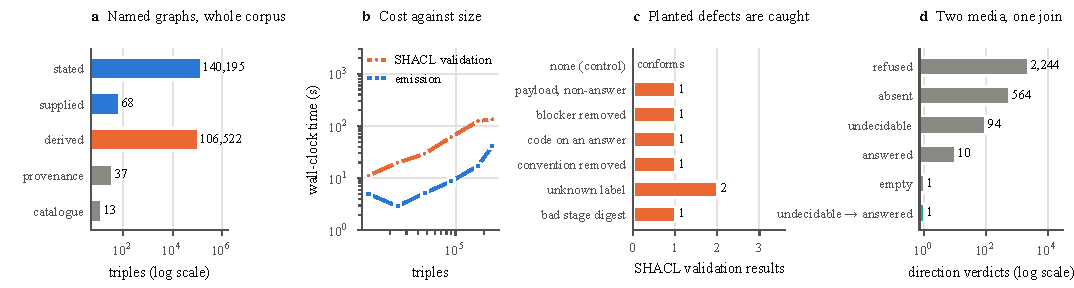
\includegraphics[width=\textwidth]{figures/fig_extension.pdf}
\caption{The DCAT-AP-PLUS extension on the full corpus.
(a) Triples per named graph of the emitted catalogue (log scale); blue graphs record the stated and supplied basis, orange the derived verdicts.
(b) Wall-clock time of emission and SHACL validation against the number of triples, for corpus prefixes and the full corpus.
(c) Validation results for the unaltered catalogue of the bundled example (the control) and for six planted defects.
(d) Direction verdicts of two runs under different media, joined on verdict IRIs with one SPARQL query; each bar is a pair of status labels (first run $\to$ second run), and the green bar is the only pair that changed.}
\label{fig:extension}
\end{figure*}


\subsection{Structure of the cytosolic network}
\label{sec:res-corpus}

With the 14 chemostatted species merged into the medium, the graph has 5{,}330 internal species and 2{,}914 reactions.
The stoichiometric matrix has rank 2{,}667, so the network has 2{,}663 conservation laws and 247 independent steady-state flux modes; the rank cut fell in a gap between $1.1\times10^{-5}$ and $10^{-15}$.
With only the medium open, 2{,}364 reactions are blocked (\cref{prop:blocked}): they carry no flux in any steady state, whatever the rate constants.
Opening the 4{,}002 boundary species, those only produced or only consumed, leaves 95 blocked.
Most cytosolic reactions are therefore fragments of pathways whose other steps lie outside the compartment or outside its annotation.

No species state is solved: 4{,}603 are \st{absent} and 727 modifiers, whose mass balance reads $0=0$, are \st{underdetermined} (\cref{fig:structure}a).
Colour refinement from the radius-1 cut key passes through nine partitions to 6{,}792 classes over 8{,}244 vertices (\cref{fig:structure}d).
Of the reactions, 537 share a class; the largest shared class has 71 members, all binding events of 14-3-3 proteins with phosphorylated partners.
Locating a vertex within its class needs 0.65 bits on average.
The graph contains 17 unbranched series chains, the longest the ten steps of retroviral reverse transcription, and all their flux control coefficients are \st{absent} for want of conductances.

\begin{figure*}[t]
\centering
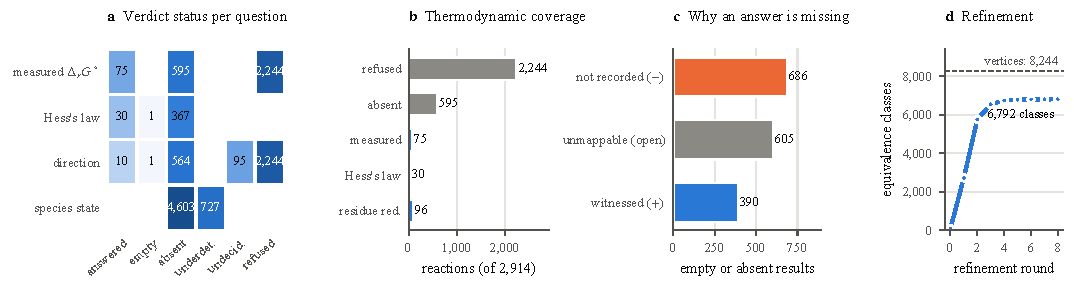
\includegraphics[width=\textwidth]{figures/fig_structure.pdf}
\caption{Structure and coverage of the cytosolic reaction network.
(a) Status of every result emitted by the extension, by question; colour is $\log_{10}$ of the count.
(b) Thermodynamic coverage of the 2{,}914 reactions; grey bars are not determined, blue bars have a chemical-reference \DG\ by measurement, Hess's law or residue reduction.
(c) Absence codes of the 1{,}681 empty or absent results of the research implementation.
(d) Weisfeiler--Leman refinement from the radius-1 cut key; the dashed line is the number of vertices.}
\label{fig:structure}
\end{figure*}

\subsection{Thermodynamic coverage}
\label{sec:res-thermo}

TECRDB contributes 418 reactions in the temperature and grade window.
Matching yields 75 reactions with a measured \DG, from 61 distinct TECRDB reactions.
Of the others, 2{,}244 are \st{refused} for a macromolecular participant and 595 are \st{absent}, 398 of them for want of a measurement and 197 for want of a KEGG identifier (\cref{fig:structure}b).
The 61 matched reactions are linearly independent, so the cycle test is \st{certified-empty}: the question is well posed and the measured reactions close no cycle.
The full TECRDB set is not consistent: the weighted Hess fit over 418 reactions and 495 compounds has $\chi^2=275.6$ on 67 degrees of freedom, a Birge ratio of 2.03 \citep{birge1932calculation}, so the quoted uncertainties are about half the scatter.

Of the 398 unmeasured small-molecule reactions, 30 lie in the span of the measured ones and are \st{answered} (\cref{prop:hess}).
One has no net chemical change, and 367 are \st{absent}: 324 contain a compound measured in no reaction and 43 lie outside the span.
Of the 2{,}244 refused reactions, 653 keep the same protein on both sides, and residue reduction answers 96 of them (94 kinase and 2 phosphatase steps).
Of the rest, 104 are \st{underdetermined} because the names state a number of sites inconsistent with the phosphoryl transfers, and 453 are \st{absent}.
Expanding the 1{,}116 catalysts gives 4{,}546 reactions over 6{,}962 species with unchanged conservation-law and flux-mode dimensions, as the expansion requires; the enzyme total is conserved for 682 catalysts and broken for 434.

\subsection{The medium and direction (M1--M3)}
\label{sec:res-medium}

Our Legendre transform reproduces eQuilibrator's on all 3{,}276 TECRDB rows in the window to $6.8\times10^{-13}\kJ$.
The comparison can fail: shifting the pH by 0.1 leaves 66 rows within $10^{-6}\kJ$, and dropping the Debye--H\"uckel term leaves 59.

\paragraph{M1, transfer between conditions (holds)}
Each condition of every TECRDB reaction measured under three or more conditions was held out and predicted from the others (\cref{fig:medium}b).
The transform model, one chemical-reference value per reaction, beats the training mean in 84 of 137 reactions in interpolation (Wilcoxon $p=8\times10^{-4}$) and in 95 of 154 in extrapolation ($p=5\times10^{-6}$).
Its advantage lies where the transform moved by more than 1\kJ\ (errors 1.95 against 2.94\kJ); where it moved less, the errors are equal.
Its mean error is 1.13 times the replicate noise of 1.38\kJ\ in interpolation and 1.88 times in extrapolation, within the stated limit of two, and in extrapolation it is no worse than an affine model in pH ($p=0.27$).
In interpolation the two-parameter affine model was better (77 against 58 reactions, $p=0.009$), which the claim did not predict.

\paragraph{M2, direction (count fails, attribution holds)}
Of the 201 reactions with a chemical value, two directions are answered, both pyrophosphate hydrolysis by the cytosolic pyrophosphatases, against a prediction of more than three.
They clear zero by 0.28\kJ.
For 156 of the other 199 (78\%), including all 96 phosphorylations, the sign of \DGm\ is fixed across the medium window, so concentrations are the missing datum; for 43 the medium window admits both signs (\cref{fig:medium}c,d).
\Cref{fig:medium}a shows such a reaction: its \DGm\ changes sign within the window of pH and free magnesium.

\paragraph{M3, crowding and dilution (both fail)}
Pyrophosphate hydrolysis adds one solute particle, and its 0.28\kJ\ margin is below the 0.92\kJ\ crowding shift at $a=0.7$, so crowding changes both decided directions.
The dilute-solution bound $2nv$ at 10\,mM has a median of 0.0035 but reaches 0.027 for a 1{,}873\,Da compound, above the stated $10^{-2}$.

\begin{figure*}[t]
\centering
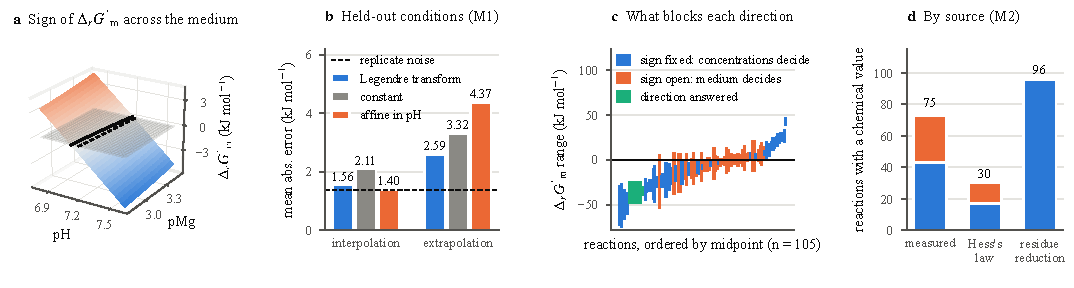
\includegraphics[width=\textwidth]{figures/fig_medium.pdf}
\caption{The cytosolic medium and the direction of reactions.
(a) At $I=0.25$\,M, \DGm\ (all participants at 1\,mM) of \MEDIUMREACTION\ over pH and pMg, as computed by the extension.
Blue is forward and orange reverse, and the grey plane is $\DGm=0$.
The lines mark the change of sign at $I=0.25$\,M (solid) and $I=0.1$\,M (dashed).
(b) Mean absolute error of held-out transformed Gibbs energies for three models (M1); the dashed line is the replicate noise between studies.
(c) Range of \DGm\ over the medium window, widened by $q\sigma$, for the \NDIRECTIONS\ reactions with a chemical value in the extension's run, coloured by what blocks the direction.
(d) Direction verdicts of the research implementation by the source of the chemical value (M2).}
\label{fig:medium}
\end{figure*}

\subsection{Proteins, binding and production routes}
\label{sec:res-proteins}

Of the phosphosites named on phosphorylation reactions, 206 were located in their protein with the named residue type, on 131 reactions and 101 proteins; attaching them adds 60{,}657 residue vertices and 222{,}072 contact edges.
Over the 60 vertices whose separation cost was computed before and after, attachment never lowered it (20 increases), as \cref{prop:monotone} requires.
The control, which replaced the counted attachment weights by real-valued residue exposures, lowered it for 46.
Named sites are more exposed than residues of the same type in the same proteins (Mann--Whitney $p=0.0049$): no named site is buried, against 3.1\% of the comparison residues.

From the metabolite's side, binding is negligible: the median bound-to-free ratio of 161 metabolites is 0.001--0.003, and only 8 exceed one (\cref{fig:proteins}c).
From the enzyme's side, it is not: over 223 enzymes, the median $c^\ast$ is 2.4\,\textmu M, 76 depart below 1\,\textmu M, and 221 depart by more than 10\% at 1\,mM (\cref{fig:proteins}b).
Enzyme--substrate complexes therefore cannot be folded into metabolite capacitances, and must stay explicit with conserved enzyme totals.

\paragraph{K1, descriptors and $K_m$ (holds)}
Under leave-one-protein-out validation over 272 proteins and 1{,}228 pairs, a ridge map from five AlphaFold descriptors did not improve on the substrate mean of $\log_{10}K_m$ (mean errors 0.780 and 0.775; one-sided $p=0.94$).
A planted effect of 0.5 standard deviations was detected ($p=0.007$).

\paragraph{Production routes}
Over 540 sources and 779 targets (420{,}120 pairs), most pairs have no route, because most reactions need a second small molecule (\cref{fig:proteins}d).
Allowing reactions to run backwards halves the unique routes from 659 to 352 and lets the medium and proteins alone make 159{,}614 targets instead of 56{,}088.
Fixing the 158 directions whose sign is fixed adds 38 unique routes (11\%) and removes 18{,}331 pairs from those made without the source.

\begin{figure*}[t]
\centering
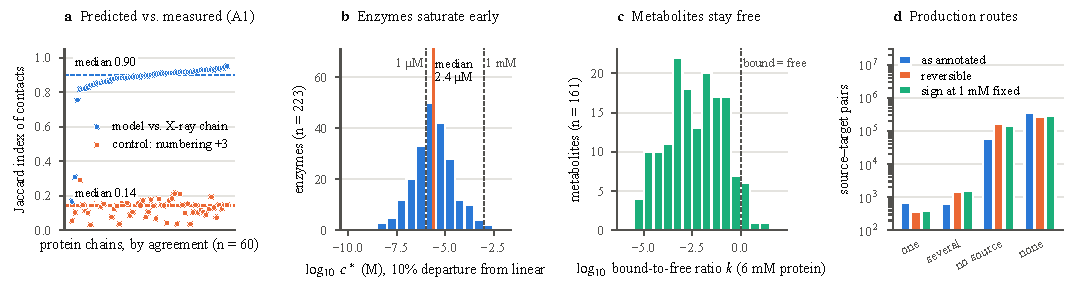
\includegraphics[width=\textwidth]{figures/fig_proteins.pdf}
\caption{Proteins, binding and production routes.
(a) Jaccard index of residue contact sets between AlphaFold models and X-ray chains (blue) and after shifting one numbering by three residues (orange, the control); dashed lines are medians (A1).
(b) Substrate concentration $c^\ast$ at which an enzyme's occupancy departs by 10\% from the linear regime, for 223 enzymes with measured $K_m$.
(c) Bound-to-free ratio of 161 metabolites at total enzyme, with 6\,mM total protein.
(d) Outcomes of the production-route search under three direction semantics (log scale).}
\label{fig:proteins}
\end{figure*}

\subsection{A coupled-oscillator account of folding (F1--F5)}
\label{sec:res-folding}

We tested an account in which residues are Kuramoto phase oscillators \citep{kuramoto1984chemical} coupled by a matrix $K$, secondary structure appears as phase-locked groups, and the number of large eigenvalues of $K$ counts secondary-structure elements.
Its motivation is Levinthal's argument that folding is not an unbiased search \citep{levinthal1969fold,dill2012folding}.
Every test was run with a coupling from sequence alone, $K_{\mathrm{seq}}$, and with the AlphaFold contact graph, $K_{\mathrm{AF}}$.
Secondary structure was assigned from backbone hydrogen bonds \citep{kabsch1983dssp}, which agreed with authors' records per residue at 0.83--0.91 in four crystal structures, against 0.24--0.42 for shuffled residues.
On 607 high-confidence models, $K_{\mathrm{seq}}$ reached a top-$L$ contact precision of 0.81 times the base rate, worse than random, where a hydrophobicity product reached 2.36 (F1, a reproduction).
The eigenvalue count matched the number of elements in 0 ($K_{\mathrm{seq}}$) and 3 ($K_{\mathrm{AF}}$) of 149 proteins, against 23 for a length-only baseline (F2 fails).
Phase-locked groups scored an adjusted Rand index of 0.067, against 0.486 for equal contiguous blocks (F3 fails), and the dynamics added nothing to the coupling they ran on ($p=0.14$).
Named phosphosites had lower local order than same-type residues (0.912 against 0.936, $p=0.012$; F4a holds), and not within confidence strata ($p=0.39$ and 0.13; F4b holds, weakly).
F5, a measurement, found that hierarchical ternary addresses bound distance but miss 45\% of contacts that straddle a cell boundary.

\subsection{Database cross-checks (E1--E6, R1--G1)}
\label{sec:res-db}

\paragraph{Absence codes and modifiers (E1--E3, measurements)}
All 1{,}681 empty or absent results of the research implementation carry an absence code: 686 not recorded, 605 unmappable and 390 witnessed (\cref{fig:structure}c).
Of 175 inhibitor edges, 147 are macromolecular partners and \st{refused}, 26 small molecules have no inhibition constant and 2 no KEGG compound; no modifier edge is answered.
Of 168 branch points, 3 have every sibling's $k_{\mathrm{cat}}$, $K_m$ and abundance.
One of their shares, glucose between aldose reductase (0.52) and hexokinases (0.48), is not credible, since hexokinases saturate at millimolar glucose.

\paragraph{Redox couples and labels (E4--E6)}
From the Hess span, the NAD and NADP couples lie 1.6\,mV apart (E4a holds), and the reduction of glutathione disulfide (GSSG) to reduced glutathione (GSH), NADPH + GSSG $\to$ NADP$^+$ + 2\,GSH, has $\DGp=-13.8\kJ$, inside the predicted $-16\pm10\kJ$ (E4b holds).
E4c, that the electron-transfer rate from the flavin--cysteine distance exceeds $k_{\mathrm{cat}}$ in glutathione and thioredoxin reductase \citep{moser1992nature,page1999natural}, could not be tested: SABIO-RK has no human wild-type $k_{\mathrm{cat}}$ for either.
Enzyme Commission (EC) labels split 4 of 147 shared structural classes, against 53.7 for shuffled labels ($p=0.005$; E5 holds).
Six stoichiometric rules assign an enzyme class from the reaction alone and agree with the EC class in 593 of 634 reactions (93.5\%, against 32.5\% shuffled; E6 holds).

\paragraph{Curated resources (R1--G1)}
For 62 reactions mapped to a directional Rhea reaction and with a fixed sign of \DGm, the sign agrees with Rhea in 45 (72.6\%), below the predicted 80\% (R1 fails).
The 17 disagreements, including triose-phosphate isomerase, glyceraldehyde-3-phosphate dehydrogenase and creatine kinase, all run uphill at 1\,mM and proceed because product is removed.
MetaNetX gave 36 more species a KEGG compound and unblocked 34 of 197 reactions (17\%, against a predicted quarter; I1 fails), but only one gained a measurement; the other 33 changed absence code from \textsf{open} to $-$.
Of 2{,}134 catalysts, 95.1\% of those with data have cytosol support (L1 holds); the 78 reactions without any supported catalyst, such as those of secreted fibrinogen chains, are candidate annotation errors.
Located phosphosites coincide with a UniProt phospho-residue in 168 of 206 cases (81.6\%; S1 holds), 141 with experimental evidence.
Catalytic residues are contact hubs, with a median of 55 heavy-atom contacts against 43 for same-type residues ($p=2.7\times10^{-18}$; a random same-type sample gives $p=0.46$; C1 holds).
AlphaFold contact sets agree with X-ray chains at a median Jaccard index of 0.90 over 60 proteins, against 0.14 for the shifted control (A1 holds; \cref{fig:proteins}a).
Outside measured disordered regions, named sites still have lower local order ($p=0.0012$; D1 fails), so disorder does not explain the F4 effect.
All 324 reactions matched to Human-GEM by participant set have the same coefficients (G1 holds), but only the 23 with a coefficient other than one could have failed.

\Cref{tab:outcomes} lists the 23 claims: 14 held, 8 failed and 1 could not be tested.
\begin{table*}[t]
\centering
\caption{Outcomes of the 23 pre-registered claims. ``Record'' is the identifier in the repository's prediction file, and ``Commit'' the commit that recorded the claim before its code was written.}
\label{tab:outcomes}
\footnotesize
\begin{tabularx}{\textwidth}{@{}lll>{\raggedright\arraybackslash}Xl>{\raggedright\arraybackslash}p{5.0cm}@{}}
\toprule
ID & Record & Commit & Claim & Outcome & Key result \\
\midrule
M1  & M1  & \texttt{de6f210} & the Legendre transform transfers between conditions & holds & error 1.13$\times$ (interpolation) and 1.88$\times$ (extrapolation) the replicate noise \\
M2a & M2  & \texttt{de6f210} & more than 3 reactions receive a direction & fails & 2 answered \\
M2b & M2  & \texttt{de6f210} & concentrations, not the medium, block most of the rest & holds & 156 of 199 \\
M3a & M3  & \texttt{de6f210} & crowding changes at most 5\% of decided directions & fails & 2 of 2 changed \\
M3b & M3  & \texttt{de6f210} & dilute bound below $10^{-2}$ for every metabolite at 10\,mM & fails & largest 0.027 \\
K1  & P1  & \texttt{de6f210} & AlphaFold descriptors do not improve $K_m$ prediction & holds & $p=0.94$; planted effect $p=0.007$ \\
F2  & F2  & \texttt{d77d09c} & eigenvalue count equals the number of secondary-structure elements & fails & 0 and 3 exact, against 23 for length alone \\
F3  & F3  & \texttt{d77d09c} & phase-locked groups beat contiguous blocks & fails & adjusted Rand index 0.067 against 0.486 \\
F4a & F4  & \texttt{d77d09c} & phosphosites have lower local order & holds & $p=0.012$ \\
F4b & F4  & \texttt{d77d09c} & no difference within confidence strata & holds (weak) & $p=0.39$ and $0.13$ \\
E4a & X4a & \texttt{cddf153} & NAD and NADP couples within 10\,mV & holds & 1.6\,mV \\
E4b & X4b & \texttt{cddf153} & NADPH reduces GSSG with $\DGp$ in $-16\pm10\kJ$ & holds & $-13.8\kJ$ \\
E4c & X4c & \texttt{cddf153} & electron-transfer rate exceeds $k_{\mathrm{cat}}$ & untestable & no $k_{\mathrm{cat}}$ in SABIO-RK \\
E5  & X5  & \texttt{cddf153} & EC labels split fewer classes than shuffled labels & holds & 4 against 53.7; $p=0.005$ \\
E6  & X6  & \texttt{cddf153} & stoichiometric rules agree with EC classes above 60\% and the null & holds & 93.5\% against 32.5\% \\
R1  & R1  & \texttt{b1d7fc8} & sign of \DGm\ agrees with the curated direction above 80\% & fails & 72.6\% \\
I1  & X1  & \texttt{b1d7fc8} & MetaNetX unblocks at least a quarter of 197 reactions & fails & 34 (17\%) \\
L1  & L1  & \texttt{b1d7fc8} & at least 80\% of catalysts have cytosol support & holds & 95.1\% \\
S1  & S1  & \texttt{b1d7fc8} & at least 70\% of sites on phospho-residues; offsets explain a third of mismatches & holds & 81.6\%; 5 of 9 \\
C1  & C1  & \texttt{b1d7fc8} & catalytic residues have more contacts & holds & $p=2.7\times10^{-18}$; control $p=0.46$ \\
A1  & P1  & \texttt{b1d7fc8} & median contact Jaccard at least 0.6; shifted control below 0.2 & holds & 0.90; 0.14 \\
D1  & D1  & \texttt{b1d7fc8} & outside measured disorder, sites do not have lower order & fails & $p=0.0012$ \\
G1  & G1  & \texttt{b1d7fc8} & Human-GEM coefficients agree in at least 90\% & holds & 324 of 324 (23 discriminating) \\
\bottomrule
\end{tabularx}
\end{table*}


%==============================================================================
\section{Discussion}
\label{sec:discussion}

\subsection{What typed results provide}
\label{sec:disc-verdicts}

An inference engine asked for the Gibbs energies of 2{,}914 reactions returns 75 values and silence.
The model returns 2{,}914 verdicts and resolves the silence by cause.
For 2{,}244 reactions the question is outside what TECRDB can state, for 398 no measurement exists, and for 197 the question cannot even be put, because a participant has no identifier TECRDB uses.
The three populations need different remedies: a different model, a measurement, and a cross-reference.
I1 shows how far the last goes: MetaNetX moved 33 reactions from the third population to the second and none to the answered set, a movement that the absence codes made visible.

V1 did real work.
A missing \DG\ never became zero, a missing $K_m$ never a typical value, and an undecided direction never the curated one.
Basis and provenance class answer a different question, what kind of value a result is.
AlphaFold contact graphs are modelled; A1 shows that they agree with measured structures, which licenses their use but does not make them measurements, and the provenance class keeps saying so.

\subsection{Concentrations are the binding constraint}
\label{sec:disc-conc}

Three results point to the same missing datum.
For 78\% of the undecided directions the medium fixes the sign of \DGm, so only concentrations remain (M2b).
The curated directions that disagree with that sign belong to reactions pulled uphill by product removal (R1).
Fixing those signs adds 11\% unique production routes.
A curated direction is thus a statement about the physiological concentration regime rather than about the reaction, and measured absolute concentrations \citep{bennett2009absolute,park2016concentrations} are the most valuable addition; a loader for them exists, its data do not.

\subsection{Implications for DCAT-AP-PLUS}
\label{sec:disc-schema}

Building the extension exposed five points where the base profiles do not yet fit a computed biochemical result.
\begin{enumerate}[leftmargin=*,itemsep=1pt,topsep=2pt]
  \item \emph{Dataset attributes.} A DCAT-AP-PLUS dataset has no slot for quantitative or qualitative attributes; they belong to activities and evaluated entities. Verdicts therefore attach to a subclass of the dataset through a new slot.
  \item \emph{Column semantics.} A quantitative attribute is a QUDT quantity with one required numeric value, so it cannot describe a table column of many values. A variable-measured construct, as in CSV on the Web or Schema.org, would close this gap.
  \item \emph{Setting.} A surrounding is defined as the place where the generating activity occurred, such as a laboratory. The cytosolic medium fits it only by extension; a class for the conditions of a biological compartment would be cleaner.
  \item \emph{Reactions.} A Chem-DCAT-AP reaction describes a reaction in a vessel, with reactor, solvent, yield, temperature and pressure, but no compartment, catalyst role or reversibility. The extension adds these.
  \item \emph{Prefixes.} Chem-DCAT-AP writes the core schema's prefix in two spellings, so offline resolution must key its import map by the expanded IRI. Unifying the prefix would remove a trap for every downstream profile.
\end{enumerate}

\subsection{Limitations}
\label{sec:limitations}

\paragraph{Scope}
The corpus follows Reactome's compartment annotation, so transport and every multi-compartment reaction are excluded, and L1 found 78 reactions whose catalysts lack cytosol support.
The extension does not yet carry residue reduction, protein contact graphs, binding or production routes; these remain in the research implementation, and kinetics are outside the extension's intended scope.

\paragraph{Thermodynamic data}
Only 61 distinct measured reactions match the corpus and close no cycle, and the wider TECRDB set is over-dispersed by a factor of about two.
The pooled uncertainty is applied uniformly.
Transforms are evaluated at 298.15\,K because TECRDB values are not temperature-corrected.
The research implementation evaluated the concentration term at 310\,K, the extension at 298.15\,K, and the difference decides eight cyclic-AMP hydrolyses (\cref{sec:res-extension}); like the pyrophosphatase directions, they lie within one convention of the boundary.

\paragraph{Conventions}
The medium window, concentration window, chemostat list, protein conversion and accessible-volume range are typical cytosolic values, not measurements for a cell type.
Each is named on every value it affects and enters the stage digest, but a different choice changes the numbers, as the comparison of two media shows.

\paragraph{Statistics}
The 23 claims were tested at $\alpha=0.05$ without correction, as declared.
Most decisive outcomes are far from the threshold, but F4a ($p=0.012$) would not survive a Bonferroni correction and should be read as suggestive.
Each stage was run once on fixed data.
One implementation fault was found and is reported: the UniProt parser first truncated notes at semicolons, which lowered S1 from 81.6\% to 19\% until it was fixed.

\paragraph{Data access}
Measured concentration tables, the Human Metabolome Database, the BRaunschweig ENzyme DAtabase (BRENDA) and PhosphoSitePlus could not be obtained under their terms by scripted download \citep{park2016concentrations,wishart2022hmdb,chang2021brenda,hornbeck2015psp}; their loaders return \st{absent} and name the missing file.

%==============================================================================
\section{Conclusion}
\label{sec:conclusion}

A knowledge graph of biochemistry need not infer.
When its edges carry constitutive relations, its structure yields rank, conservation laws, blocked reactions and cycle constraints without a parameter.
When its answers are typed results with provenance that cannot be laundered, every gap is named by cause and every remedy is explicit.
The DCAT-AP-PLUS extension described here makes these properties part of the metadata: they are declared in a LinkML schema, checked by SHACL shapes and carried in PROV-O named graphs.
Any consumer can therefore verify them, and two runs can be compared result by result.
Applied to the human cytosol, the model shows how little public measurements determine, 105 reaction energies by measurement and Hess's law and a handful of directions, and what would determine more.
Concentrations would decide most directions, measurement rather than identifiers limits thermodynamic coverage, and enzyme saturation rather than metabolite binding governs the contacts.

%==============================================================================
\section*{Data and code availability}
The extension is the Python package \breakingtt{dcat-ap-plus-homo-sapien}, version 0.1.0a1, at \url{https://git.uni-greifswald.de/sachikonyk/dcat-ap-plus-homo-sapien} (MIT licence).
The research implementation \texttt{circuit\_kg} is on branch \texttt{circuit-kg} of \url{https://github.com/fullscreen-triangle/nebuchadnezzar}; its results are from commit \texttt{15fb81a}, and the claims were committed in \texttt{de6f210}, \texttt{d77d09c}, \texttt{cddf153} and \texttt{b1d7fc8}, each before the code that tested them.
Every downloaded file is recorded with its address, retrieval date and SHA-256 digest.
Every number in this paper is read from the results files, and the figures and the extension's measurements are produced by the scripts in the manuscript's directory (\ref{app:reproduce}).

\section*{Acknowledgements}
This work was carried out within NFDI4Cat, which is funded by the Deutsche Forschungsgemeinschaft (DFG).
The author thanks the maintainers of Reactome, ChEBI, TECRDB, eQuilibrator, SABIO-RK, PaxDb, UniProt, the AlphaFold Protein Structure Database, the Protein Data Bank, Rhea, MetaNetX, Human-GEM, the Human Protein Atlas, COMPARTMENTS, M-CSA and DisProt for making their data openly available.

\section*{Declaration of competing interest}
The author declares no competing interests.

\bibliographystyle{elsarticle-num}
\bibliography{refs}

\appendix
%==============================================================================
\section{Named conventions}
\label{app:conventions}

Every supplied value names the convention that produced it (\cref{tab:conventions}).
The extension declares those it uses as \term{hs:Convention} plans in the supplied graph and associates each with the run.

\begin{table*}[t]
\centering
\caption{Conventions supplied by the research implementation. Those marked $\ast$ are registered by the extension, which declares each one it uses as a PROV-O plan.}
\label{tab:conventions}
\footnotesize
\newcolumntype{C}{>{\raggedright\arraybackslash\ttfamily\hyphenchar\font=`\-}p{3.3cm}}%
\begin{tabularx}{\textwidth}{@{}C>{\raggedright\arraybackslash}XC>{\raggedright\arraybackslash}X@{}}
\toprule
\normalfont Convention & Meaning & \normalfont Convention & Meaning \\
\midrule
ambient-reservoir$^\ast$ & the 14 cofactors of \cref{sec:graph} are chemostatted and merged into the medium &
slot-from-name$^\ast$ & modified residues are read from Reactome species names \\
medium-floor$^\ast$ & every vertex has a medium edge of weight 1 &
enzyme-cycle-2$^\ast$ & each catalysed reaction becomes a binding and a catalytic step \\
modifier-unit-weight$^\ast$ & every modifier edge has weight 1 &
medium-floor-residue & a buried residue still receives a medium edge of weight 1 \\
conjugate-closure$^\ast$ & a KEGG compound reached through conjugate acids, bases and tautomers &
protein-ppm-to-molar$^\ast$ & PaxDb parts per million times 2--6\,mM total protein molecules \\
water-balance$^\ast$ & a TECRDB match that holds once water is balanced &
scope-from-source$^\ast$ & a route may use the source, the medium and the proteins no reaction makes \\
concentration-window$^\ast$ & 1\,\textmu M to 10\,mM for every metabolite &
dilute-limit-share$^\ast$ & a branch's share is $(k_{\mathrm{cat}}/K_m)[E]$ over its siblings' sum \\
medium-window$^\ast$ & pH 6.8--7.6, ionic strength 0.1--0.25\,M, pMg 2.8--3.5, 298.15\,K &
loss-of-function-variant$^\ast$ & Reactome's ``Defective \dots'' reactions are modifiers on their wild-type edge \\
accessible-volume$^\ast$ & $\mu=\mu^\circ+RT\ln(c/a)$ with $a\in[0.7,1]$ for every small solute &
textbook-standard-conditions & redox couples at pH 7, $I=0.25$\,M, 298.15\,K, no magnesium \\
hess-span$^\ast$ & a \DG\ derived from measured reactions by Hess's law &
moser-dutton-defaults & reorganisation energy 0.7\,eV, driving force 0, packing density 0.76 \\
pH-window & pH 6.8 to 7.6 (first stage only) &
medium-as-slowest-rung & a chain's medium resistance equals its slowest step's \\
carrier-slot$^\ast$ & a protein unchanged across a reaction adds nothing to its \DG &
mnx-xref & a KEGG compound reached through MetaNetX where conjugate closure found none \\
free-residue$^\ast$ & a residue in a protein reacts like the free amino acid &
measured-window$^\ast$ & a per-compound concentration window from a declared table \\
kegg-candidate-selected-by-tecrdb-match$^\ast$ & one of several KEGG candidates, selected because exactly one combination matches &
brenda-same-reference & a BRENDA $k_{\mathrm{cat}}$ pairs with a $K_m$ of the same protein, substrate and reference \\
\bottomrule
\end{tabularx}
\end{table*}

%==============================================================================
\section{Reproduction}
\label{app:reproduce}

\paragraph{Research implementation}
From the root of the repository, the stages run in order as \texttt{python -m circuit\_kg} with the subcommands \texttt{fetch}, \texttt{extract}, \texttt{build} (about 13\,min, mostly singular value decompositions), \texttt{proteins}, \texttt{attach}, \texttt{medium}, \texttt{kinetics}, \texttt{complete}, \texttt{folding}, \texttt{extend} and \texttt{databases}.
Each writes one results file.
The first run of a network-dependent stage downloads and caches its sources.
The 53 tests run with \texttt{python -m pytest circuit\_kg/tests}.

\paragraph{Extension}
\texttt{uv sync} installs the extension with its development dependencies, and \texttt{uv run pytest} runs its 89 tests, nine of which execute the example notebooks.
The command line offers \texttt{summary}, \texttt{emit -o catalogue.trig}, \texttt{validate catalogue.trig} (exit status 1 on a violation) and \texttt{reactome} to read an SBML export into the corpus exchange format.

\paragraph{This manuscript}
\texttt{scripts/full\_inputs.py} writes the extension's inputs for the full corpus from the research implementation's prepared data.
\texttt{scripts/extension\_audit.py}, run in the extension's environment, writes \texttt{data/extension.json}.
\texttt{scripts/make\_numbers.py} turns it and the research implementation's results into the macros and the reproduction table used in the text.
\texttt{figures/make\_figures.py} draws all four figures from the results files, and no number is typed in.

%==============================================================================
\section{Text of the claims}
\label{app:claims}

The claims are given as recorded, with identifiers mapped as in \cref{tab:outcomes}.
Each states what would count against it.

\begin{description}[style=unboxed,leftmargin=0pt,itemsep=2pt,font=\normalfont\bfseries]
\item[M1] On TECRDB reactions measured under three or more conditions, hold out one condition at a time. The transform model's mean absolute error approaches the replicate noise and is below the constant model's.
Its largest advantage is where the held-out transform moved by more than 1\kJ; in extrapolation it is no worse than an affine model in pH. \emph{Against:} error above twice the replicate noise, no advantage where the medium moved, or the affine model better in extrapolation.
\item[M2] More than the first stage's 3 reactions receive a direction (M2a). For most of the rest the sign of \DGm\ is fixed across the medium window, so the blocker is the concentration window (M2b). \emph{Against:} for most reactions the medium window alone admits both signs.
\item[M3] Crowding with $a\in[0.7,1]$ changes at most a few directions (M3a), and the dilute bound stays below $10^{-2}$ per particle for every metabolite at 10\,mM (M3b). \emph{Against:} more than 5\% of decided directions change, or the bound exceeds $10^{-2}$.
\item[K1] Under leave-one-protein-out validation, a ridge map from five AlphaFold descriptors does not reduce the error of a substrate baseline for $\log_{10}K_m$ (one-sided Wilcoxon $p\ge0.05$). \emph{Against:} $p<0.05$ with lower mean error.
\item[F2] The number of eigenvalues of $K$ above $\lambda_c=K_0e^{-1/2}\bar L$ equals the number of secondary-structure elements. \emph{Against:} an exact-match rate no higher than a length-only baseline.
\item[F3] Phase-locked groups from $K_{\mathrm{AF}}$ beat equal contiguous blocks per protein (one-sided Wilcoxon $p<0.05$).
\item[F4] Named sites have lower local order than same-type residues (F4a); within confidence strata below 70 and at least 70 the difference has one-sided $p\ge0.05$ (F4b).
\item[E4] The NAD and NADP couples lie within 10\,mV (E4a), and \DGp\ of NADPH + GSSG $\to$ NADP$^+$ + 2\,GSH is within 10\kJ\ of $-16\kJ$ (E4b).
For glutathione reductase and thioredoxin reductase~1 the electron-transfer rate from the flavin--cysteine edge distance exceeds the measured $k_{\mathrm{cat}}$, and a control at 25\,\AA\ falls below it (E4c). A value that cannot be derived is recorded as \st{absent}, not as a failure.
\item[E5] Real EC labels split fewer shared structural classes than labels shuffled among the same reactions (200 shuffles, $p<0.05$).
\item[E6] On reactions whose catalyst has a single EC class, the stoichiometric class agrees with it in more than 60\% of classifiable reactions and above a shuffle null.
\item[R1] For reactions mapped to a directional Rhea reaction, a fixed sign of \DGm\ agrees with Rhea's direction in more than 80\%.
\item[I1] MetaNetX supplies a KEGG compound for a participant in at least a quarter of the 197 reactions blocked by a missing identifier.
\item[L1] At least 80\% of catalysts have cytosol support in the Human Protein Atlas or COMPARTMENTS (confidence at least 3).
\item[S1] At least 70\% of the 206 located phosphosites coincide with a UniProt phospho-residue, and one numbering offset per protein explains at least a third of the 9 residue mismatches.
\item[C1] M-CSA catalytic residues have more heavy-atom contacts than same-type residues in the same AlphaFold models (one-sided Mann--Whitney $p<0.05$).
\item[A1] For proteins with an experimental structure covering at least 80\% of a high-confidence AlphaFold model, the median Jaccard index of contact sets is at least 0.6, and shifting the numbering by 3 residues drops it below 0.2.
\item[D1] Outside DisProt disordered regions, named sites do not have lower local order than same-type residues (one-sided $p\ge0.05$).
\item[G1] Where a reaction's small-molecule participants equal those of a Human-GEM cytosolic reaction, the coefficients agree in at least 90\%.
\end{description}


\end{document}
